\documentclass{../../../oss-apphys}

\begin{document}
\genheader

\gentitle{1}{ROTATIONAL MOTION}

\genmultidirections

\gengravity

\raggedcolumns
\begin{multicols}{2}
  \begin{enumerate}[leftmargin=18pt]
  \item Linear acceleration is to force as angular acceleration is to
    \begin{enumerate}[noitemsep,topsep=0pt,leftmargin=18pt,label=(\Alph*)]
    \item kinetic energy
    \item angular velocity
    \item rotational inertia
    \item torque
    \item angular momentum
    \end{enumerate}

  \item A meter stick of mass \SI{.1}{\kilo\gram} rests on a table as shown. A
    length of \SI{40}{\centi\metre} extends over the edge of the table. How far
    from the edge of the table could a \SI{.05}{\kilo\gram} mass be placed on
    the meter stick so that the stick just begins to tip?
    \begin{center}
      \vspace{-.2in}
      \pic{.28}{beam1.png}
    \end{center}
    \begin{enumerate}[noitemsep,topsep=0pt,leftmargin=18pt,label=(\Alph*)]
    \item\SI{5}{\centi\metre}
    \item\SI{10}{\centi\metre}
    \item\SI{15}{\centi\metre}
    \item\SI{20}{\centi\metre}
    \item\SI{30}{\centi\metre}
    \end{enumerate}
    
  \item A meter stick is balanced on a fulcrum at its center, as shown. A mass
    of \SI{5}{\kilo\gram} is hung on the left end of the stick, and a mass of
    \SI{2}{\kilo\gram} is hung on the right end. In order to balance the
    system, a mass $m$ is hung at the 25-cm mark on the right
    side. What is the value of the mass $m$?
    \begin{center}
      \pic{.33}{beam2.png}
    \end{center}
    \begin{enumerate}[noitemsep,topsep=0pt,leftmargin=18pt,label=(\Alph*)]
    \item\SI{12}{\kilo\gram}
    \item\SI{6 }{\kilo\gram}
    \item\SI{4 }{\kilo\gram}
    \item\SI{3 }{\kilo\gram}
    \item\SI{2 }{\kilo\gram}
    \end{enumerate}
    
  \item A metal bar of constant density and weight $W$ is attached to a pivot on
    the wall at point $P$ and supported by a rope that makes an angle of
    \ang{60} with the vertical wall. The reaction force exerted by the pivot on
    the bar at point P is best represented by which arrow?
    \begin{center}
      \pic{.25}{metal-bar.png}
    \end{center}
    \begin{enumerate}[noitemsep,topsep=0pt,leftmargin=18pt,label=(\Alph*)]
    \item\vspace{-.15in} $\nearrow$
    \item $\uparrow$
    \item $\downarrow$
    \item $\nwarrow$
    \item $\searrow$
    \end{enumerate}

  \item A uniform rod of length $L$ and mass $m$ has a rotational inertia of
    $\displaystyle \frac1{12}mL^2$ about its center. A particle, also of mass
    $m$, is attached to one end of the stick. The combined rotational inertia of
    the stick and particle about the center of the rod is
    \begin{center}
      \pic{.3}{I.png}
    \end{center}
    \begin{enumerate}[noitemsep,topsep=0pt,leftmargin=18pt,label=(\Alph*)]
    \item$\displaystyle\frac{mL^2}{3}$
    \item$\displaystyle\frac{12mL^2}{13}$
    \item$\displaystyle\frac{13mL^2}{12}$
    \item$\displaystyle\frac{mL^2}{156}$
    \item$\displaystyle\frac{13mL^2}{156}$
    \end{enumerate}
%    \columnbreak

  \item A hoop of radius $R$ and mass $m$ has a rotational inertia of $mR^2$.
    The hoop rolls without slipping along a horizontal floor with a constant
    speed $v$ and then rolls up a long incline. The hoop can roll up the
    incline to a maximum vertical height of
    \begin{center}
      \pic{.4}{hoop1.png}
    \end{center}
    \begin{enumerate}[noitemsep,topsep=0pt,leftmargin=18pt,label=(\Alph*)]
    \item$\displaystyle\frac{v^2}{g}$
    \item$\displaystyle\frac{2v^2}{g}$
    \item$\displaystyle\frac{v^2}{2g}$
    \item$\displaystyle\frac{4v^2}{g}$
    \item$\displaystyle\frac{v^2}{4g}$
    \end{enumerate}
    
  \item Two disks are fixed to a vertical axle that is rotating with a constant
    angular speed $\omega$. The smaller disk has a mass $m$ and a radius $r$,
    and the larger disk has a mass $2m$ and radius $2r$. The general equation
    for the rotational inertia of a disk of mass $M$ and radius $R$ is
    $\frac12MR^2$. The ratio of the angular momentum of the larger disk to
    the smaller disk is
    \begin{center}
      \pic{.25}{2disks.png}
    \end{center}
    \begin{enumerate}[noitemsep,topsep=0pt,leftmargin=18pt,label=(\Alph*)]
    \item$1:4$
    \item$4:1$
    \item$1:2$
    \item$2:1$
    \item$8:1$
    \end{enumerate}
    \columnbreak
    
  \item A light rod has a mass attached at each end. At one end is a
    \SI{6}{\kilo\gram} mass, and at the other end is a \SI{3}{\kilo\gram} mass.
    An axis can be placed at any of the points shown. Through which point
    should an axis be placed so that the rotational inertia is the greatest
    about that axis?
    \begin{center}
      \pic{.4}{light-rod.png}
    \end{center}
    \begin{enumerate}[noitemsep,topsep=0pt,leftmargin=18pt,label=(\Alph*)]
    \item A
    \item B
    \item C
    \item D
    \item E
    \end{enumerate}
    
%  \item Two wheels are attached to each other and fixed so that they can only
%    turn together. The smaller wheel has a radius of $r$ and the larger wheel
%    has a radius of $3r$. The two wheels can rotate together on a frictionless
%    axle. Three forces act tangentially on the edge of the wheels as shown.
%    The magnitude of the net torque acting on the system of wheels is
%    \begin{center}
%      \pic{.25}{2wheels.png}
%    \end{center}
%    \begin{enumerate}[noitemsep,topsep=0pt,leftmargin=18pt,label=(\Alph*)]
%    \item$Fr$
%    \item$2Fr$
%    \item$3Fr$
%    \item$4Fr$
%    \item$6Fr$
%    \end{enumerate}

    
  \item Astronauts are conducting an experiment in a negligible gravity
    environment. Two spheres of mass $m$ are attached to either end of a light
    rod. As the rod and spheres float motionless in space, an astronaut
    launches a piece of sticky clay, also of mass $m$, toward one of the spheres
    so that the clay strikes and sticks to the sphere perpendicular to the rod.
    Which of the following statements is true of the motion of the rod, clay,
    and spheres after the collision?
    \begin{center}
      \pic{.25}{collision1.png}
    \end{center}
    \begin{enumerate}[noitemsep,topsep=0pt,leftmargin=18pt,label=(\Alph*)]
    \item Linear momentum is not conserved, but angular momentum is conserved.
    \item Angular momentum is not conserved, but linear momentum is conserved.
    \item Kinetic energy is conserved, but angular momentum is not conserved.
    \item Kinetic energy is conserved, but linear momentum is not conserved.
    \item Both linear momentum and angular momentum are conserved, but kinetic
      energy is not conserved.
    \end{enumerate}
    \columnbreak
    
  \item One end of a stick of length $L$, rotational inertia $I$, and mass $m$
    is pivoted on an axle with negligible friction at point $P$. The other end
    is tied to a string and held in a horizontal position. When the string is
    cut, the stick rotates counterclockwise. The angular speed $\omega$ of the
    stick when it reaches the bottom of its swing is
    \begin{center}
      \pic{.4}{end-of-stick.png}
    \end{center}
    \begin{enumerate}[noitemsep,topsep=0pt,leftmargin=18pt,label=(\Alph*)]
    \item$\displaystyle\frac{mgL}{I}$
    \item$\displaystyle\sqrt{\frac{mgL}{I}}$
    \item$\displaystyle\sqrt{\frac{2mgL}{I}}$
    \item$\displaystyle\sqrt{\frac{mgL}{2I}}$
    \item$\displaystyle\sqrt{\frac{4mgL}{I}}$
    \end{enumerate}

  \item A disk is mounted on a fixed axle. The rotational inertia of the disk is
    $I$. The angular velocity of the disk is decreased from $\omega_0$ to
    $\omega_f$ during a time $\Delta t$ due to friction in the axle. The
    magnitude of the average net torque acting on the wheel is
    \begin{enumerate}[noitemsep,topsep=0pt,leftmargin=18pt,label=(\Alph*)]
    \item $\displaystyle\frac{\omega_f-\omega_0}{\Delta t}$
    \item $\displaystyle\frac{(\omega_f-\omega_o)^2}{\Delta t}$
    \item $\displaystyle\frac{I(\omega_f-\omega_o)}{\Delta t}$
    \item $\displaystyle\frac{I(\omega_f-\omega_o)^2}{\Delta t}$
    \item $\displaystyle\frac{I(\omega_f-\omega_o)}{\Delta t^2}$
    \end{enumerate}
    \columnbreak
    
  \item The average power developed by the friction in the axle of the disk
    from the previous question to bring it to a complete stop is
    \begin{enumerate}[noitemsep,topsep=0pt,leftmargin=18pt,label=(\Alph*)]
    \item $\displaystyle\frac{\omega_o}{\Delta t}$
    \item $\displaystyle\frac{(\omega_o)^2}{\Delta t}$
    \item $\displaystyle\frac{I(\omega_f-\omega_o)}{2\Delta t}$
    \item $\displaystyle\frac{I\omega_o^2}{2\Delta t}$
    \item $\displaystyle\frac{I(\omega_f-\omega_o)}{\Delta t^2}$
    \end{enumerate}
    
  \item A light rod of negligible mass is pivoted at point $P$ a distance $L$
    from one end as shown. A mass $m$ is attached to the left end of the rod at
    a distance of $3L$ from the pivot, and another mass $4m$ is attached to the
    other end a distance $L$ from the pivot. The system begins from rest in the
    horizontal position. The net torque acting on the system due to
    gravitational forces is
    \begin{center}
      \pic{.4}{light-rod2.png}
    \end{center}
    \begin{enumerate}[noitemsep,topsep=0pt,leftmargin=18pt,label=(\Alph*)]
    \item $4mgL$ clockwise
    \item $3mgL$ clockwise
    \item $3mgL$ counterclockwise
    \item $mgL$ counterclockwise
    \item $mgL$ clockwise
    \end{enumerate}
    
  \item The angular acceleration of the system when it is released from rest is
    \begin{enumerate}[noitemsep,topsep=0pt,leftmargin=18pt,label=(\Alph*)]
    \item zero
    \item $\displaystyle\frac{g}{5L}$
    \item $\displaystyle\frac{g}{4L}$
    \item $\displaystyle\frac{g}{13L}$
    \item  $\displaystyle\frac{g}{L}$
    \end{enumerate}
    \columnbreak
    
  \item A satellite orbits the Earth in an elliptical orbit, with point A being
    close to the Earth and point B farther away. As the satellite moves from
    point A to point B, which of the following is true of the angular momentum
    and kinetic energy of the satellite?
    \begin{center}
      \vspace{-.1in}
      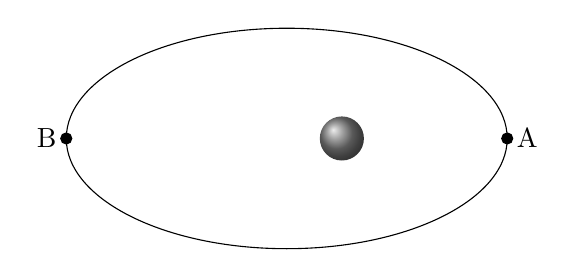
\begin{tikzpicture}[scale=1.4]
        \tikzstyle{balloon}=[ball color=gray];
        \draw(0,0) ellipse (2 and 1);
        \draw[fill=black](2,0) circle(0.05) node[right]{A};
        \draw[fill=black](-2,0) circle(0.05) node[left]{B};
        \shade[balloon] (0.5,0) circle (0.2);
      \end{tikzpicture}
    \end{center}
  
    \begin{tabular}{lll}
      & \underline{Angular momentum} & \underline{Kinetic energy}\\
      (a) & Increases & Remains constant \\
      (b) & Remains constant & Increases \\
      (c) & Decreases & Remains constant \\
      (d) & Remains constant & Decreases \\
      (e) & Remains constant & Remains constant
    \end{tabular}

  \item A moon orbits a large planet in an elliptical orbit, with its closest
    approach at a distance $a$, and its farthest distance $b$. The speed of the
    moon at point b is $v$. The speed at point $a$ is
    \begin{enumerate}[noitemsep,topsep=0pt,leftmargin=18pt,label=(\Alph*)]
    \item $\displaystyle\frac{av}{b}$
    \item $\displaystyle\frac{bv}{a}$
    \item $\displaystyle\frac{(a+b)v}{b}$
    \item $\displaystyle\frac{(b-a)v}{b}$
    \item $\displaystyle\frac{2bv}{a}$
    \end{enumerate}
    \columnbreak
    
  \item A satellite orbits the Earth in an elliptical orbit. Which of the
    following statements is true?
    \begin{enumerate}[noitemsep,topsep=0pt,leftmargin=18pt,label=(\Alph*)]
    \item The angular velocity of the satellite increases as it travels farther
      from the Earth.
    \item The acceleration of the satellite increases as it travels closer to
      the Earth.
    \item The angular momentum of the satellite increases as it travels closer
      to the Earth.
    \item The potential energy of the satellite is equal to its kinetic energy
      at all points in the orbit.
    \item The speed of the satellite must remain constant for it to remain
      in orbit around the Earth.
    \end{enumerate}

  \item Two moons of mass $m$ and $2m$ orbit a planet of mass $M$ at the same
    radius $R$ and speed $v$ toward each other, as shown. The moons collide and
    stick together without destroying either moon. The total momentum of the
    moons after the collision is
    \begin{center}
      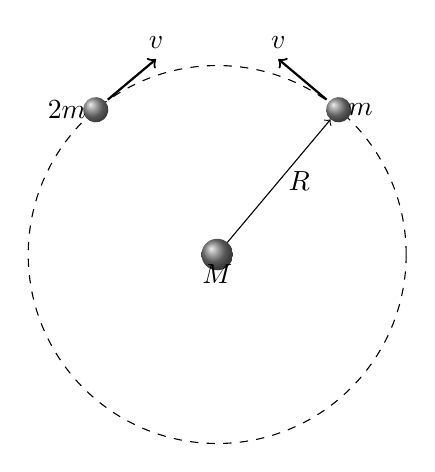
\begin{tikzpicture}[scale=0.8]
        \tikzstyle{balloon}=[ball color=gray];
        \shade[balloon] circle(.25) node[below]{$M$};
        \draw[dashed](0,0) circle(3);
        \begin{scope}[rotate=50]
          \draw[->](0.25,0)--(2.8,0) node[midway,right]{$R$};
          \shade[balloon] (3,0) circle (0.2) node[right]{$m$};
          \draw[thick,->](3,0.25)--(3,1.25) node[pos=1,above]{$v$};
        \end{scope}
        \begin{scope}[rotate=130]
          \shade[balloon] (3,0) circle (0.2) node[left]{$2m$};
          \draw[thick,->](3,-0.25)--(3,-1.25) node[pos=1,above]{$v$};
        \end{scope}
      \end{tikzpicture}
    \end{center}
    \begin{enumerate}[noitemsep,topsep=0pt,leftmargin=18pt,label=(\Alph*)]
    \item $mv$
    \item $2mv$
    \item $3mv$
    \item $6mv$
    \item zero
    \end{enumerate}    
  \end{enumerate}
\end{multicols}

\newpage
%\genanswersheet{1 \& C}{Simple Harmonic Motion and Universal Gravitation}
%
%\begin{center}
%  \begin{minipage}[t]{.2\textwidth}
%    \vspace{.2in}
%    \bgroup
%    \begin{tabular}{>{\centering}m{1.3cm} >{\centering}m{1.7cm}}
%      No. & Answer
%    \end{tabular}\\
%    \def\arraystretch{1.5}
%    \begin{tabular}{|>{\centering}m{1.3cm}|>{\centering}m{1.7cm}|}
%      \hline
%      1 & \\ \hline
%      2 & \\ \hline
%      3 & \\ \hline
%      4 & \\ \hline
%      5 & \\ \hline
%      6 & \\ \hline
%      7 & \\ \hline
%      8 & \\ \hline
%      9 & \\ \hline
%      10 & \\ \hline
%      11 & \\ \hline
%      12 & \\ \hline
%      13 & \\ \hline
%      14 & \\ \hline
%      15 & \\ \hline
%      16 & \\ \hline
%      17 & \\ \hline
%      18 & \\ \hline
%      19 & \\ \hline
%      20 & \\ \hline
%      21 & \\ \hline
%      22 & \\ \hline
%      23 & \\ \hline
%      24 & \\ \hline
%      25 & \\ \hline
%    \end{tabular}
%    \egroup
%  \end{minipage}
%  \hspace{.5in}
%  \begin{minipage}[t]{.2\textwidth}
%    \vspace{.2in}
%    \bgroup
%    \begin{tabular}{>{\centering}m{1.3cm} >{\centering}m{1.7cm}}
%      No. & Answer
%    \end{tabular}\\
%    \def\arraystretch{1.5}
%    \begin{tabular}{|>{\centering}m{1.3cm}|>{\centering}m{1.7cm}|}
%      \hline
%      26 & \\ \hline
%      27 & \\ \hline
%      28 & \\ \hline
%      29 & \\ \hline
%      30 & \\ \hline
%      31 & \\ \hline
%      32 & \\ \hline
%      33 & \\ \hline
%      34 & \\ \hline
%      35 & \\ \hline
%      36 & \\ \hline
%      37 & \\ \hline
%      38 & \\ \hline
%    \end{tabular}
%    \egroup
%  \end{minipage}
%\end{center}
%\newpage

\genfreetitle{1}{ROTATIONAL MOTION}{5}

\genfreedirections

% TAKEN FROM THE 2016 AP PHYSICS 1 EXAM FREE-RESPONSE QUESTION #1
\begin{center}
  \pic{.4}{wooden-wheel1.png}
\end{center}

\begin{enumerate}[leftmargin=15pt]
\item A wooden wheel of mass $M$, consisting of a rim with spokes, rolls down
  a ramp that makes an angle $\theta$ with the horizontal, as shown above. The
  ramp exerts a force of static friction on the wheel so that the wheel rolls
  without slipping.
  \begin{enumerate}[leftmargin=15pt,noitemsep]
  \item
    \begin{enumerate}[leftmargin=15pt,noitemsep]
    \item On the diagram below, draw and label the forces (not components) that
      act on the wheel as it rolls down the ramp, which is indicated by the
      dashed line. To clearly indicate at which point on the wheel each force
      is exerted, draw each force as a distinct arrow starting on, and pointing
      away from, the point at which the force is exerted. The lengths of the
      arrows need not indicate the relative magnitudes of the forces.
      \begin{center}
        \pic{.22}{wooden-wheel2.png}
      \end{center}
    \item As the wheel rolls down the ramp, which force causes a change in the
      angular velocity of the wheel with respect to its center of mass? Briefly
      explain your reasoning.
      \vspace{.7in}
    \end{enumerate}

  \item For this ramp angle, the force of friction exerted on the wheel is less
    than the maximum possible static friction force. Instead, the magnitude of
    the force of static friction exerted on the wheel is 40 percent of the
    magnitude of the force or force component directed opposite to the force of
    friction. Derive an expression for the linear acceleration of the wheel's
    center of mass in terms of $M$, $\theta$, and physical constants, as
    appropriate.
    \newpage
    
  \item In a second experiment on the same ramp, a block of ice, also with mass
    $M$, is released from rest at the same instant the wheel is released from
    rest, and from the same height. The block slides down the ramp with
    negligible friction.
    \begin{enumerate}[leftmargin=15pt,noitemsep]
    \item Which object, if either, reaches the bottom of the ramp with the
      greatest speed?

      \vspace{.1in}
      \underline{\hspace{.3in}} Wheel\hspace{.2in}
      \underline{\hspace{.3in}} Block\hspace{.2in}
      \underline{\hspace{.3in}} Neither; both reach the bottom with the same
      speed.

      \vspace{.1in}Briefly explain your answer, reasoning in terms of forces.
      
    \item Briefly explain your answer again, now reasoning in terms of energy.
    \end{enumerate}
  \end{enumerate}
  \vspace{1.5in}

  % TAKEN FROM THE 2018 AP PHYSICS 1 EXAM FREE-RESPONSE QUESTION #1
  \begin{center}
    \pic{.4}{spacecraft1}\\
    \underline{Note:} Figure not drawn to scale.
  \end{center}
\item A spacecraft of mass $m$ is in a clockwise circular orbit of radius $R$
  around Earth, as shown in the figure above. The mass of Earth is $M_E$.
  \begin{enumerate}[leftmargin=15pt,noitemsep]
  \item In the figure below, draw and label the forces (not components) that
    act on the spacecraft. Each force must be represented by a distinct arrow
    starting on, and pointing away from, the spacecraft.
    \begin{center}
      \pic{.3}{spacecraft2}\\
      \underline{Note:} Figure not drawn to scale.
  \end{center}

  \item
    \begin{enumerate}[leftmargin=15pt,noitemsep]
    \item Derive an equation for the orbital period $T$ of the spacecraft in
      terms of $m$, $M_E$, $R$, and physical constants, as appropriate. If you
      need to draw anything other than what you have shown in part (a) to
      assist in your solution, use the space below. Do NOT add anything to the
      figure in part (a).
      \vspace{1in}
    \item A second spacecraft of mass $2m$ is placed in a circular orbit with
      the same radius $R$. Is the orbital period of the second spacecraft
      greater than, less than, or equal to the orbital period of the first
      spacecraft?

      \vspace{.1in}
      \underline{\hspace{.3in}}Greater than\hspace{.2in}
      \underline{\hspace{.3in}}Less than\hspace{.2in}
      \underline{\hspace{.3in}}Equal to
      
      \vspace{.1in}Briefly explain your reasoning.
      \vspace{.5in}
    \end{enumerate}
    
  \item The first spacecraft is moved into a new circular orbit that has a
    radius greater than $R$, as shown in the figure below.
    \begin{center}
      \pic{.3}{spacecraft3}\\
      \underline{Note:} Figure not drawn to scale.
    \end{center}
    Is the speed of the spacecraft in the new orbit greater than, less than, or
    equal to the original speed?
    
    \vspace{.1in}
    \underline{\hspace{.3in}}Greater than\hspace{.2in}
    \underline{\hspace{.3in}}Less than\hspace{.2in}
    \underline{\hspace{.3in}}Equal to
      
    \vspace{.1in}Briefly explain your reasoning.   
  \end{enumerate}
  \newpage
  
  \begin{center}
    \pic{.4}{disk1}
  \end{center}
\item The disk shown above spins about the axle at its center. A student's
  experiments reveal that, while the disk is spinning, friction between the
  axle and the disk exerts a constant torque on the disk.
  \begin{enumerate}[leftmargin=15pt]
  \item At time $t=0$ the disk has an initial counterclockwise (positive)
    angular velocity $\omega_0$. The disk later comes to rest at time $t=t_1$.
    \begin{enumerate}[leftmargin=15pt]
    \item On the grid at left below, sketch a graph that could represent the
      disk's angular velocity as a function of time $t$ from $t=0$ until the
      disk comes to rest at time $t=t_1$.   
    \item On the grid at right below, sketch the disk's angular acceleration as
      a function of time $t$ from $t=0$ until the disk comes to rest at time
      $t=t_1$.   
    \end{enumerate}
    \begin{center}
    \pic{.9}{graph1}
  \end{center}
  \item The magnitude of the frictional torque exerted on the disk is
    $\tau_0$ . Derive an equation for the rotational inertia $I$ of the disk in
    terms of $\tau_0$, $\omega_0$, $t_1$, and physical constants, as
    appropriate.
    \vspace{.75in}
    \newpage
    
  \item In another experiment, the disk again has an initial positive angular
    velocity $\omega_0$ at time $t=0$. At $\displaystyle t=\frac12t_1$, the
    student starts dripping oil on the contact surface between the axle and the
    disk to reduce the friction. As time passes, more and more oil reaches that
    contact surface, reducing the friction even further.
    %time t =
     \begin{enumerate}[leftmargin=15pt]
     \item On the grid at left below, sketch a graph that could represent the
       disk's angular velocity as a function of time from $t=0$ to $t=t_1$,
       which is the time at which the disk came to rest in part (a).
     \item On the grid at right below, sketch the disk's angular acceleration
       as a function of time from $t=0$ to $t=t_1$.
     \end{enumerate}
     \begin{center}
       \pic{.9}{graph2}
     \end{center}
   \item The student is trying to mathematically model the magnitude $\tau$ of
     the torque exerted by the axle on the disk when the oil is present at
     times $\displaystyle t>\frac12t_1$. The student writes down the following
     two equations, each of which includes a positive constant ($C_1$ or $C_2$)
     with appropriate units.
     \begin{enumerate}[label={(\arabic*)},leftmargin=15pt]
     \item$\displaystyle\tau=C_1\left(t-\frac12t_1\right)$ (for $t>\frac12 t_1$)
     \item$\displaystyle\tau=\frac{C_2}{\left(t+\frac12t_1\right)}$ (for
       $t>\frac12t_1$)
     \end{enumerate}
     Which equation better mathematically models this experiment?

     \vspace{.1in}
     \underline{\hspace{.3in}}Equation (1)\hspace{.2in}
     \underline{\hspace{.3in}}Equation (2)
     
     \vspace{.1in}Briefly explain why the equation you selected is plausible
     and why the other equation is not plausible.
  \end{enumerate}
%\item Two stars of unequal mass orbit each other about their common center of
%  mass as shown. The star of mass $M_1$ orbits in a circle of radius $r$, and
%  the star of mass $M_2$ orbits in a circle of radius $2r$.
%  \begin{center}
%    \begin{tikzpicture}[scale=0.8]
%      \tikzstyle{balloon}=[ball color=gray];
%      \draw[fill=black](0,0) circle(0.075);
%      \draw[dashed](0,0) circle(3);
%      \draw[dashed](0,0) circle(1.5);
%      \draw[->](0,0)--(1.5,0) node[midway,below]{$r$};
%      \shade[balloon] (1.5,0) circle (0.2) node[right]{$M_1$};
%      \draw[->](0,0)--(-3,0) node[midway,below]{$2r$};
%      \shade[balloon] (-3,0) circle (0.2) node[left]{$M_2$};
%    \end{tikzpicture}
%  \end{center}
%  \begin{enumerate}[noitemsep,leftmargin=20pt]
%  \item Determine the ratio of masses $M_1/M_2$.
%  \item Determine the ratio of the acceleration $a_1$ of $M_1$ to the
%    acceleration $a_2$ of $M_2$.
%  \item Determine the ratio of the period $T_1$ of $M _1$ to the period $T_2$
%    of $M_2$.
%  \end{enumerate}
%  \vspace{2.2in}
%  
%\item As a member of the 2240 Olympic Committee, you are considering a new
%  sport: asteroid jumping. On Earth, world-class high jumpers routinely clear
%  \SI{2}{\metre}. Your job is to make sure athletes jumping from asteroids will
%  return to the asteroid. Make the simplifying assumption that asteroids are
%  spherical, with an average density of \SI{2500}{\kilo\gram\per\metre^3}. For
%  safety, make sure that even a jumper capable of \SI{3}{\metre} on Earth will
%  return to the surface. What do you report for the minimum asteroid diameter?
%  \newpage
%
%\item Two point particles of mass $m$ are on the $y$ axis at $y=a$ and $y=-a$,
%  as shown in the figure below.
%  \begin{center}
%    \begin{tikzpicture}[scale=.8]
%      \tikzstyle{balloon1}=[ball color=green!50!gray];
%      \tikzstyle{balloon2}=[ball color=red!50];
%      \draw[->](-2,0)--(6,0) node[pos=1,right]{$x$};
%      \draw[->](0,-3)--(0,3) node[pos=1,above]{$y$};
%      \draw[<->](-1,0)--(-1,2) node[midway,left]{$a$};
%      \draw[<->](-1,0)--(-1,-2)node[midway,left]{$a$};
%      \draw(0,2)--(-1.2,2);
%      \draw(0,-2)--(-1.2,-2);
%      \shade[balloon1] (0,2) circle (.55) node[white]{$m$};
%      \shade[balloon1] (0,-2)circle (.55) node[white]{$m$};
%      \shade[balloon2] (4,0) circle (.45) node[white]{$m_0$};
%    \end{tikzpicture}
%  \end{center}
%  \begin{enumerate}[noitemsep,leftmargin=20pt]
%  \item Derive the expression for the gravitational force exerted by these two
%    particles on a third particle of mass $m_0$ located on teh $x$ axis at a
%    distance $x$ away from the origin.
%  \item What is the gravitational field $\mb{g}$ on the $x$-axis due to the
%    two particles?
%  \item Show that $g_x$ (the $x$ component of $\mb{g}$) due to the two
%    particles on the $y$ axis is approximately $\displaystyle-\frac{2Gm}{x^2}$
%    when $x$ is much greater than $a$.
%  \item Show that the maximum value of $|g_x|$ occurs at the point
%    $\displaystyle x=\frac{\pm a}{\sqrt{2}}$.
%  \end{enumerate}
%  \newpage
%
%\item Five equal masses $M$ are equally spaced on the arc of a semicircle of
%  radius $R$ as shown in the figure below. A mass $m$ is located at the center
%  of curvature of the arc. If $M$ is \SI{3}{\kilo\gram}, $m$ is
%  \SI{21}{\kilo\gram}, nad $R$ is \SI{10}{\centi\metre}, what is the force on
%  $m$ due to the five masses?
%  \begin{center}
%    \begin{tikzpicture}[scale=.8]
%      \tikzstyle{balloon1}=[ball color=gray!50];
%      \tikzstyle{balloon2}=[ball color=red!60!black];
%      \draw[->](0,0)--(5,0) node[pos=1,right]{$x$};
%      \draw[->](0,0)--(0,5) node[pos=1,above]{$y$};
%      \draw[ultra thick,blue!80](4,0) arc(0:180:4);
%      \shade[balloon1] (0,0) circle (.1) node[below]{$m$};
%      \foreach \theta in {0,45,...,180} {
%        \begin{scope}[rotate=\theta]
%          \shade[balloon2] (4,0) circle (.3) node[white]{$M$};
%        \end{scope}
%      }
%    \end{tikzpicture}
%  \end{center}
\end{enumerate}
\end{document}
